%%%%%%%%%%%%%%%%%%%%%%%%%%%%%%%%%%%%%%%%%%%%%%%%%%%%%%%%%%%%%%%%%%%%%%%%%%
%Author:																 %
%-------																 %
%Yannis Baehni at University of Zurich									 %
%baehni.yannis@uzh.ch													 %
%																		 %
%Version log:															 %
%------------															 %
%06/02/16 . Basic structure												 %
%04/08/16 . Layout changes including section, contents, abstract.		 %
%%%%%%%%%%%%%%%%%%%%%%%%%%%%%%%%%%%%%%%%%%%%%%%%%%%%%%%%%%%%%%%%%%%%%%%%%%

%Page Setup
\documentclass[
	12pt, 
	oneside, 
	a4paper,
	reqno,
	final
]{amsart}

\usepackage[
	left = 3cm, 
	right = 3cm, 
	top = 3cm, 
	bottom = 3cm
]{geometry}

\usepackage{mathptmx}

%Headers and footers
\usepackage{fancyhdr}
	\pagestyle{fancy}
	%Clear fields
	\fancyhf{}
	%Header right
	\fancyhead[R]{
		\footnotesize
		Yannis B\"{a}hni\\
		\href{mailto:yannis.baehni@uzh.ch}{yannis.baehni@uzh.ch}
	}
	%Header left
	\fancyhead[L]{
		\footnotesize
		Internship in Numerics\\
		Autumn 2017
	}
	%Page numbering in footer
	\fancyfoot[C]{\thepage}
	%Separation line header and footer
	\renewcommand{\headrulewidth}{0.4pt}
	%\renewcommand{\footrulewidth}{0.4pt}
	
	\setlength{\headheight}{19pt} 
\usepackage{graphicx}
\usepackage{subcaption}
%Title
\usepackage[foot]{amsaddr}
\usepackage{upref}
\usepackage{amssymb}
\usepackage{mathrsfs}
\DeclareMathAlphabet{\mathscrbf}{OMS}{mdugm}{b}{n}
%\usepackage{mathptmx}
\usepackage{xspace}
\makeatletter
\def\@textbottom{\vskip \z@ \@plus 1pt}
\let\@texttop\relax
\usepackage{etoolbox}
\patchcmd{\abstract}{\scshape\abstractname}{\textbf{\abstractname}}{}{}

\usepackage[all,cmtip]{xy}

%Section, subsection and subsubsection font
%------------------------------------------
\makeatletter
	\renewcommand{\@secnumfont}{\bfseries}
	\renewcommand\section{\@startsection{section}{1}%
  	\z@{.7\linespacing\@plus\linespacing}{.5\linespacing}%
  	{\normalfont\bfseries\centering}}
	\renewcommand\subsection{\@startsection{subsection}{2}%
    	\z@{.5\linespacing\@plus.7\linespacing}{-.5em}%
    	{\normalfont\bfseries}}%
	\renewcommand\subsubsection{\@startsection{subsubsection}{3}%
    	\z@{.5\linespacing\@plus.7\linespacing}{-.5em}%
    	{\normalfont\bfseries}}%
%Formatting title of TOC
\renewcommand{\contentsnamefont}{\bfseries}
%Table of Contents
\setcounter{tocdepth}{3}

% Add bold to \section titles in ToC and remove . after numbers
\renewcommand{\tocsection}[3]{%
  \indentlabel{\@ifnotempty{#2}{\bfseries\ignorespaces#1 #2\quad}}\bfseries#3}
% Remove . after numbers in \subsection
\renewcommand{\tocsubsection}[3]{%
  \indentlabel{\@ifnotempty{#2}{\ignorespaces#1 #2\quad}}#3}
\let\tocsubsubsection\tocsubsection% Update for \subsubsection
%...

\newcommand\@dotsep{4.5}
\def\@tocline#1#2#3#4#5#6#7{\relax
  \ifnum #1>\c@tocdepth % then omit
  \else
    \par \addpenalty\@secpenalty\addvspace{#2}%
    \begingroup \hyphenpenalty\@M
    \@ifempty{#4}{%
      \@tempdima\csname r@tocindent\number#1\endcsname\relax
    }{%
      \@tempdima#4\relax
    }%
    \parindent\z@ \leftskip#3\relax \advance\leftskip\@tempdima\relax
    \rightskip\@pnumwidth plus1em \parfillskip-\@pnumwidth
    #5\leavevmode\hskip-\@tempdima{#6}\nobreak
    \leaders\hbox{$\m@th\mkern \@dotsep mu\hbox{.}\mkern \@dotsep mu$}\hfill
    \nobreak
    \hbox to\@pnumwidth{\@tocpagenum{\ifnum#1=1\bfseries\fi#7}}\par% <-- \bfseries for \section page
    \nobreak
    \endgroup
  \fi}
\AtBeginDocument{%
\expandafter\renewcommand\csname r@tocindent0\endcsname{0pt}
}
\def\l@subsection{\@tocline{2}{0pt}{2.5pc}{5pc}{}}
\def\l@subsubsection{\@tocline{2}{0pt}{4.5pc}{5pc}{}}
\makeatother

\advance\footskip0.4cm
\textheight=54pc    %a4paper
\textheight=50.5pc %letterpaper
\advance\textheight-0.4cm
\calclayout

%Font settings
%\usepackage{anyfontsize}
%Footnote settings
%\usepackage{mathptmx}
\usepackage{footmisc}
%	\renewcommand*{\thefootnote}{\fnsymbol{footnote}}
\usepackage{commath}
%Further math environments
%Further math fonts (loads amsfonts implicitely)
\usepackage{amssymb}
%Redefinition of \text
%\usepackage{amstext}
\usepackage{upref}
%Graphics
%\usepackage{graphicx}
%\usepackage{caption}
%\usepackage{subcaption}
%Frames
\usepackage{mdframed}
\allowdisplaybreaks
%\usepackage{interval}
\newcommand{\toup}{%
  \mathrel{\nonscript\mkern-1.2mu\mkern1.2mu{\uparrow}}%
}
\newcommand{\todown}{%
  \mathrel{\nonscript\mkern-1.2mu\mkern1.2mu{\downarrow}}%
}
\AtBeginDocument{\renewcommand*\d{\mathop{}\!\mathrm{d}}}
\renewcommand{\Re}{\operatorname{Re}}
\renewcommand{\Im}{\operatorname{Im}}
\DeclareMathOperator\Log{Log}
\DeclareMathOperator\Arg{Arg}
\DeclareMathOperator\sech{sech}
\DeclareMathOperator*\esssup{ess.sup}
\DeclareMathOperator\id{id}
\DeclareMathOperator\res{res}
\let\div\undefined
\DeclareMathOperator\div{div}
\DeclareMathOperator\sgn{sgn}
%\usepackage{hhline}
%\usepackage{booktabs} 
%\usepackage{array}
%\usepackage{xfrac} 
%\everymath{\displaystyle}
%Enumerate
\usepackage{tikz}
\usetikzlibrary{external}
\tikzexternalize % activate!
\usetikzlibrary{patterns}
\pgfdeclarepatternformonly{adjusted lines}{\pgfqpoint{-1pt}{-1pt}}{\pgfqpoint{40pt}{40pt}}{\pgfqpoint{39pt}{39pt}}%
{
  \pgfsetlinewidth{.8pt}
  \pgfpathmoveto{\pgfqpoint{0pt}{0pt}}
  \pgfpathlineto{\pgfqpoint{39.1pt}{39.1pt}}
  \pgfusepath{stroke}
}
\usepackage{enumitem} 
%\renewcommand{\labelitemi}{$\bullet$}
%\renewcommand{\labelitemii}{$\ast$}
%\renewcommand{\labelitemiii}{$\cdot$}
%\renewcommand{\labelitemiv}{$\circ$}
%Colors
%\usepackage{color}
%\usepackage[cmtip, all]{xy}
%Theorems
\newtheoremstyle{bold}              	 %Name
  {}                                     %Space above
  {}                                     %Space below
  {\itshape}		                     %Body font
  {}                                     %Indent amount
  {\bfseries}                             %Theorem head font
  {.}                                    %Punctuation after theorem head
  { }                                    %Space after theorem head, ' ', 
  										 %	or \newline
  {\thmname{#1}\thmnumber{ #2}\thmnote{ (#3)}} 
\theoremstyle{bold}
\newtheorem*{definition*}{Definition}
\newtheorem{definition}{Definition}[section]
\newtheorem*{lemma*}{Lemma}
\newtheorem{lemma}{Lemma}[section]
\newtheorem{Proof}{Proof}[section]
\newtheorem{proposition}{Proposition}[section]
\newtheorem{properties}{Properties}[section]
\newtheorem{corollary}{Corollary}[section]
\newtheorem*{theorem*}{Theorem}
\newtheorem{theorem}{Theorem}[section]
\newtheoremstyle{solution}              	 %Name
{}                                     %Space above
{}                                     %Space below
{}		      			               %Body font
{}                                     %Indent amount
{\bfseries}                             %Theorem head font
{.}                                    %Punctuation after theorem head
{ }                                    %Space after theorem head, ' ', 
%	or \newline
{\thmname{#1}\thmnumber{ #2}\thmnote{ (#3)}} 
\theoremstyle{solution}
\newtheorem*{solution}{Lösung}
\newtheorem{remark}{Remark}[section]
\newtheorem{examples}{Examples}[section]
\newtheorem{example}{Example}[section]
\newtheoremstyle{exercise}              	 %Name
{}                                     %Space above
{}                                     %Space below
{\small}		      			               %Body font
{}                                     %Indent amount
{\bfseries}                             %Theorem head font
{.}                                    %Punctuation after theorem head
{ }                                    %Space after theorem head, ' ', 
%	or \newline
{\thmname{#1}\thmnumber{ #2}\thmnote{ (#3)}} 
\theoremstyle{exercise}
\newtheorem{exercise}{Aufgabe}
%German non-ASCII-Characters
%Graphics-Tool
%\usepackage{tikz}
%\usepackage{tikzscale}
%\usepackage{bbm}
%\usepackage{bera}
%Listing-Setup
%Bibliographie
\usepackage[backend=bibtex, style=alphabetic]{biblatex}
%\usepackage[babel, german = swiss]{csquotes}
\bibliography{bibliography}
%PDF-Linking
%\usepackage[hyphens]{url}
\usepackage[bookmarksopen=true,bookmarksnumbered=true]{hyperref}
%\PassOptionsToPackage{hyphens}{url}\usepackage{hyperref}
\hypersetup{
  colorlinks   = true, %Colours links instead of ugly boxes
  urlcolor     = blue, %Colour for external hyperlinks
  linkcolor    = blue, %Colour of internal links
  citecolor    = blue %Colour of citations
}
%Weierstrass-P symbol for power set
\newcommand{\powerset}{\raisebox{.15\baselineskip}{\Large\ensuremath{\wp}}}
\newcommand{\bld}[1]{\boldmath\textit{\textbf{#1}}\unboldmath}

\makeatletter
\providecommand*{\rightharpoonupfill@}{%
  \arrowfill@\relbar\relbar\rightharpoonup
}
\providecommand*{\xrightharpoonup}[2][]{%
  \ext@arrow 0579\rightharpoonupfill@{#1}{#2}%
}
\makeatother

\usepackage{listings}

\definecolor{mygreen}{rgb}{0,0.6,0}
\definecolor{mygray}{rgb}{0.5,0.5,0.5}
\definecolor{mymauve}{rgb}{0.58,0,0.82}
\lstset{ %
  backgroundcolor=\color{white},   % choose the background color; you must add \usepackage{color} or \usepackage{xcolor}; should come as last argument
  basicstyle=\scriptsize,        % the size of the fonts that are used for the code
  breakatwhitespace=false,         % sets if automatic breaks should only happen at whitespace
  breaklines=true,                 % sets automatic line breaking
  captionpos=b,                    % sets the caption-position to bottom
  commentstyle=\color{mygreen},    % comment style
  deletekeywords={...},            % if you want to delete keywords from the given language
  escapeinside={\%*}{*)},          % if you want to add LaTeX within your code
  extendedchars=true,              % lets you use non-ASCII characters; for 8-bits encodings only, does not work with UTF-8
  frame=single,	                   % adds a frame around the code
  keepspaces=true,                 % keeps spaces in text, useful for keeping indentation of code (possibly needs columns=flexible)
  keywordstyle=\color{blue},       % keyword style
  language=Octave,                 % the language of the code
  morekeywords={*,...},            % if you want to add more keywords to the set
  numbers=left,                    % where to put the line-numbers; possible values are (none, left, right)
  numbersep=5pt,                   % how far the line-numbers are from the code
  numberstyle=\tiny\color{mygray}, % the style that is used for the line-numbers
  rulecolor=\color{black},         % if not set, the frame-color may be changed on line-breaks within not-black text (e.g. comments (green here))
  showspaces=false,                % show spaces everywhere adding particular underscores; it overrides 'showstringspaces'
  showstringspaces=false,          % underline spaces within strings only
  showtabs=false,                  % show tabs within strings adding particular underscores
  stepnumber=2,                    % the step between two line-numbers. If it's 1, each line will be numbered
  stringstyle=\color{mymauve},     % string literal style
  tabsize=2,	                   % sets default tabsize to 2 spaces
  title=\lstname                   % show the filename of files included with \lstinputlisting; also try caption instead of title
}
\newcommand{\Ascr}{\mathscr{A}}
\newcommand{\pot}{\mathrm{pot}}
\begin{document}

%Remake Tikz-picture
%\tikzset{external/force remake}

\begin{abstract}

\end{abstract}

\title{Estimates of the modeling error generated by homogenization of an elliptic boundary value problem}
\author{Yannis B\"{a}hni}
\address[Yannis B\"{a}hni]{University of Zurich, R\"{a}mistrasse 71, 8006 Zurich}
\email[Yannis B\"{a}hni]{\href{mailto:yannis.baehni@uzh.ch}{yannis.baehni@uzh.ch}}
\thanks{}
\maketitle

\tableofcontents

\section{The Homogenization Problem}
We follow \cite[1--30]{jikov:homogenization:1994}.

\begin{definition}
Let $n \in \mathbb{Z}$, $n \geq 1$, and $\Omega \subseteq \mathbb{R}^n$ be a bounded domain. A vector $v \in (L^1(\Omega))^n$ is said to be the \bld{gradient of a function $u \in L^1(\Omega)$} if
\begin{equation}
\int_\Omega u \frac{\partial \varphi}{\partial x_i}\d \lambda = -\int_\Omega v_i \varphi\d \lambda
\end{equation} 
\noindent for all $\varphi \in \mathscr{C}^\infty_0(\Omega)$ and $i = 1,\dots,n$. The gradient $v$ of $u$ is denoted by $\nabla u$. 
\end{definition}

Define the Sobolev space $H^1(\Omega)$ by
\begin{equation}
H^1(\Omega) := \cbr[0]{u \in L^2(\Omega) : \nabla u \in (L^2(\Omega))^n}.
\end{equation}
$H^1(\Omega)$ equipped with the inner product
\begin{equation}
\langle u_1,u_2 \rangle_{H^1(\Omega)} := \int_\Omega u_1u_2 \d \lambda + \sum_{k = 1}^n\int_\Omega \frac{\partial u_1}{\partial x_k}\frac{\partial u_2}{\partial x_k}\d \lambda 
\end{equation}
\noindent is then a Hilbert space. We are mainly interested in the subspace
\begin{equation}
H^1_0(\Omega) := \overline{\mathscr{C}^\infty_0(\Omega)} \subseteq H^1(\Omega).
\end{equation}
The dual of $H^1_0(\Omega)$ is denoted by $H^{-1}(\Omega)$. We have that $L^2(\Omega) \hookrightarrow H^{-1}(\Omega)$.

\begin{definition}
Let $n \in \mathbb{Z}$, $n \geq 1$, $\Omega \subseteq \mathbb{R}^n$ be a bounded domain and $p \in (L^2(\Omega))^n$. The \bld{divergence of $p$}, written $\div p$, is defined to be an element of $H^{-1}(\Omega)$ satisfying
\begin{equation}
\langle \div p, \varphi \rangle_{H^1(\Omega)} = - \int_\Omega \langle p, \nabla \varphi \rangle_{\mathbb{R}^n} \d \lambda
\end{equation}
\noindent for all $\varphi \in H^1_0(\Omega)$.
\end{definition}

\begin{definition}
Let $n \in \mathbb{Z}$, $n \geq 1$. A constant positive definite matrix $A_0$ is said to be the \bld{homogenized matrix} for a periodic matrix $A \in M_n\del[0]{L^\infty(\mathbb{R}^n)}$ satisfying the condition of ellipticity
\begin{equation}
a_{ij}(x)y_iy_j \geq c\abs[0]{y}^2 \qquad \forall x,y \in \mathbb{R}^n
\label{eq:ellip_cond}
\end{equation}
\noindent and some $c > 0$, if for any bounded domain $\Omega \subseteq \mathbb{R}^n$ and any $f \in H^{-1}(\Omega)$ the solutions $u_\varepsilon$ of the Dirichlet problem 
\begin{equation}
\div(A_\varepsilon \nabla u_\varepsilon) = f \in H^{-1}(\Omega), \qquad u_\varepsilon \in H^1_0(\Omega),
\end{equation}
\noindent where $A_\varepsilon(x) := A(x/\varepsilon)$ possess the following propertiy of convergence:
\begin{equation}
u_\varepsilon \xrightharpoonup[]{H^1_0(\Omega)} u_0, \qquad A_\varepsilon \nabla u_\varepsilon \xrightharpoonup[]{L^2(\Omega)} A_0\nabla u_0,
\end{equation}
\noindent as $\varepsilon \to 0$, where $u_0$ is the solution of the Dirichlet problem
\begin{equation}
\div(A_0 \nabla u_0) = f, \qquad u_0\in H^1_0(\Omega).
\end{equation}
\end{definition}

\begin{theorem}
Let $A \in M_n\del[0]{L^\infty(\mathbb{R}^n)}$ be a periodic matrix satisfying the ellipticity condition \textup{(}\ref{eq:ellip_cond}\textup{)}. Consider the auxiliary periodic problem
\begin{equation}
\div(Av) = 0, \qquad v \in L^2_{\pot}(\Box), \qquad \langle v \rangle = \alpha \in \mathbb{R}^n
\end{equation} 
\noindent and define $A_0$ by
\begin{equation}
\langle Av \rangle = A_0 \alpha.
\end{equation}
Then $A_0$ is a homogenized matrix for $A$.
\label{thm:homogenized}
\end{theorem}

\begin{proof}
See \cite[19]{jikov:homogenization:1994}.
\end{proof}

From the proof of theorem \ref{thm:homogenized} further follows that 
\begin{equation}
A_0 = \langle A(I + \nabla N)\rangle
\end{equation}
\noindent where $\nabla N$ is the matrix with columns $\nabla N_1,\dots,\nabla N_n$ which are solutions of 
\begin{equation}
\div(A(e_k + \nabla N_k)) = 0, \qquad N_k \in H^1(\Box)
\end{equation}
\noindent for $k = 1,\dots,n$.

\begin{example}
	Let $n := 1$ and $\Omega := \intoo{0,1}$. Furthermore, for $\varepsilon > 0$ define
	\begin{equation}
		A_\varepsilon(x) := 2 + \cos\del[2]{\frac{2\pi x}{\varepsilon}}
		\label{eq:A_eps}
	\end{equation}
	\noindent and let
	\begin{equation}
	f(x) := e^{10x}.
	\end{equation}
	From (\ref{eq:A_eps}) we deduce
	\begin{equation}
		A(x) = A_\varepsilon(\varepsilon x) = 2 + \cos(2\pi x).
	\end{equation}
	Now we have to solve
	\begin{equation}
		(AN')' = A'
		\label{eq:N}
	\end{equation}
	\noindent for the periodic solution $N$ such that $\int_0^1 N = 0$. Integrating (\ref{eq:N}) yields
	\begin{equation}
		N'(x) = 1 + \frac{c}{A(x)}
	\end{equation}
	\noindent for some constant $c \in \mathbb{R}$. Hence
	\begin{equation}
		N(x) = \int_0^x N'(t) \d t = \int_0^x \del[2]{1 + \frac{c}{A(t)}}\d t
	\end{equation}
	\noindent and from the periodicity requirement $N(0) = N(1)$ we get that
	\begin{equation}
		1 = - c \int_0^1 \frac{\d x}{A(x)}.
	\end{equation}
	Using \cite[170]{fischer:funktionentheorie:2003} yields
	\begin{align*}
		\int_0^1 \frac{\d x}{A(x)} &= \int_0^1 \frac{\d x}{2 + \cos(2\pi x)} = \frac{1}{2\pi}\int_0^{2\pi} \frac{\d y}{2 + \cos(y)} = 2\sum_{\abs[0]{\zeta} < 1} \res_\zeta \del{\frac{1}{z^2 + 4z + 1}} = \frac{1}{\sqrt{3}}.
	\end{align*}
	Hence
	\begin{equation}
		\boxed{N'(x) = 1 - \frac{\sqrt{3}}{2 + \cos(2\pi x)}.}
	\end{equation}
	\noindent and
	\begin{equation}
		\boxed{N(x) = \int_0^x \del[2]{1 - \frac{\sqrt{3}}{2 + \cos(2\pi t)}} \d t.}
	\end{equation}
	\noindent since 
	\begin{equation}
	\int_0^1 N(x)\d x = \frac{1}{2}\int_0^1\sbr[2]{\int_0^1 \del[2]{1 - \frac{\sqrt{3}}{2 + \cos(2\pi t)}} \d t}\d x = 0
	\end{equation}
	\noindent by the invariance of the integrand under the mapping $t \mapsto 1 - t$. Furthermore
	\begin{equation*}
		A_0 = \int_0^1 A(x) \d x - \int_0^1 A(x)N'(x) \d x = \int_0^1 A(x) \d x - \int_0^1 A(x)\del[2]{1 - \frac{\sqrt{3}}{A(x)}} \d x = \sqrt{3}.
	\end{equation*}
	Then we have to solve
	\begin{equation}
		\del[0]{A_0u'_0}' = -f.
	\end{equation}
	Integration with respect to $x$ yields
	\begin{equation}
		u'_0(x) = -\frac{1}{\sqrt{3}}\frac{1}{10}e^{10x} + c_1
	\end{equation}
	\noindent for some constant $c_1 \in \mathbb{R}$ and thus 
	\begin{equation}
		u_0(x) = -\frac{1}{\sqrt{3}}\frac{1}{100}e^{10x} + c_1x + c_2
	\end{equation}
	\noindent for some constant $c_2 \in \mathbb{R}$. Since $u_0 \in H^1_0(\Omega)$, we have that $u_0(0) = u_0(1) = 0$ and thus we get the linear system
	\begin{equation}
		-\frac{1}{\sqrt{3}}\frac{1}{100} + c_2 = 0 \qquad\qquad  -\frac{1}{\sqrt{3}}\frac{1}{100}e^{10} + c_1 + c_2 = 0.
		\label{eq:linsys}
	\end{equation}
	\noindent Solving (\ref{eq:linsys}) yields
	\begin{equation}
		\boxed{u_0(x) = \frac{1}{\sqrt{3}}\frac{1}{100} \del[1]{(e^{10} - 1)x + 1 - e^{10x}}.}
	\end{equation}
	Since $\partial \Omega = \cbr[0]{0,1}$ it is easily seen that
	\begin{equation}
	\psi_\varepsilon(x) = \min\del[0]{1,\varepsilon^{-1}\min\del[0]{x,1 - x}}
	\end{equation}
	\noindent and so
	\begin{equation}
		\boxed{w_\varepsilon^1(x) = u_0(x) - \varepsilon \min\del[0]{1,\varepsilon^{-1}\min\del[0]{x,1 - x}}N(\varepsilon^{-1}x)u'_0(x) \qquad x \in \Omega.}	
	\end{equation}
	Lastly we have to solve
	\begin{equation}
	(A_\varepsilon u_\varepsilon')' = -f.
	\end{equation}
	Integration with respect to $x$ yields
	\begin{equation}
	u_\varepsilon'(x) = \frac{1}{A_\varepsilon(x)}\del[1]{c - \frac{1}{10}e^{10x}}
	\end{equation}
	\noindent for some $c \in \mathbb{R}$. Since $u_\varepsilon \in H^1_0(\Omega)$, we have that 
	\begin{equation}
	u_\varepsilon(x) = \int_0^x \frac{1}{A_\varepsilon(t)}\del[1]{c - \frac{1}{10}e^{10t}}\d t
	\end{equation}
	\noindent and from $u_\varepsilon(1) = 0$ we deduce
	\begin{equation}
	\boxed{u_\varepsilon(x) = \frac{1}{10}\int_0^x \frac{1}{A_\varepsilon(t)}\del[2]{\int_0^1 \frac{e^{10s}}{A_\varepsilon(s)}\d s \del[2]{\int_0^1 \frac{\d s}{A_\varepsilon(s)}}^{-1} - e^{10t}}\d t.}
	\end{equation}
	In figure \ref{fig:ex_2_plots} we see the approximations of $u_\varepsilon$ by $w_\varepsilon^1$. One observes that the approximation is even good for a relatively large choice of $\varepsilon$. 
	
	\begin{figure}[h!tb]
    \centering
    \begin{subfigure}[b]{0.5\textwidth}
        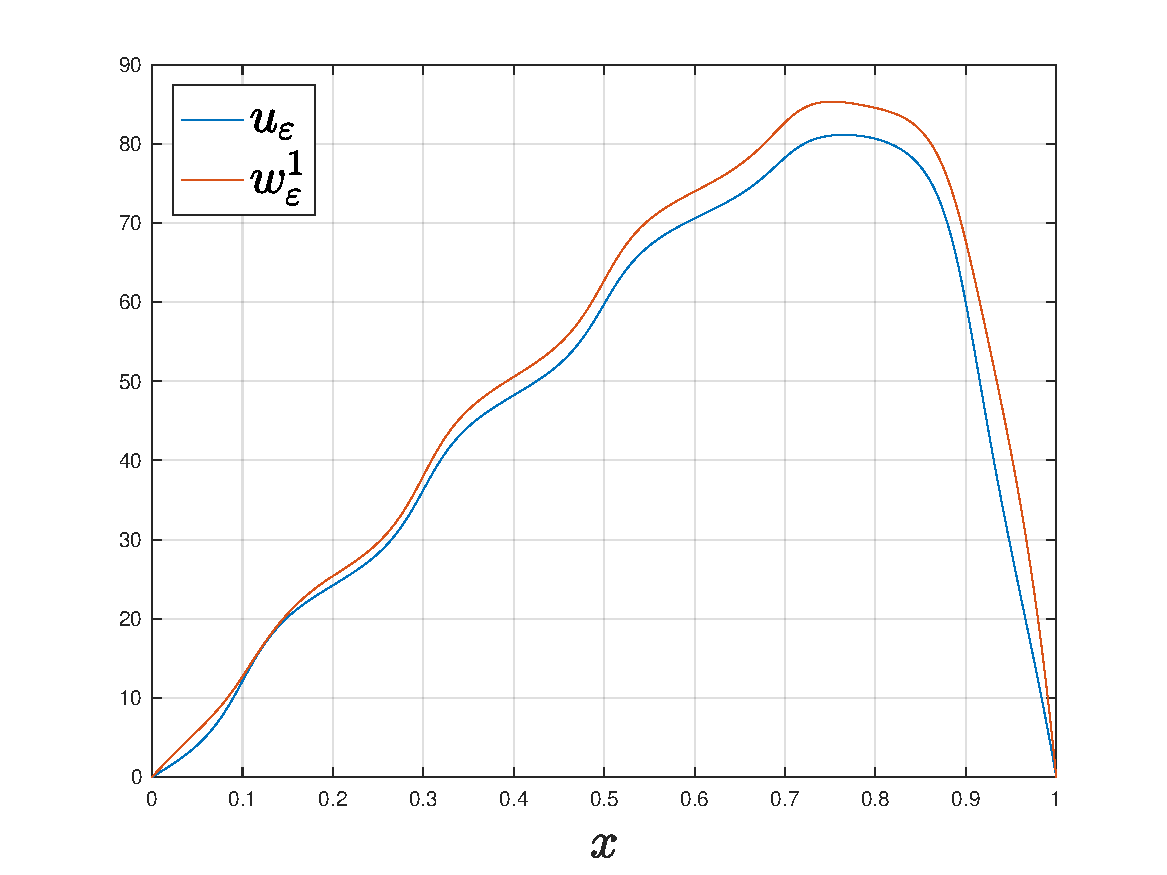
\includegraphics[width=\textwidth]{src/img/u_eps_w_1_eps_1.pdf}
        \caption{$\varepsilon = 0.2$}
    \end{subfigure}
    ~ %add desired spacing between images, e. g. ~, \quad, \qquad, \hfill etc. 
      %(or a blank line to force the subfigure onto a new line)
    \begin{subfigure}[b]{0.5\textwidth}
        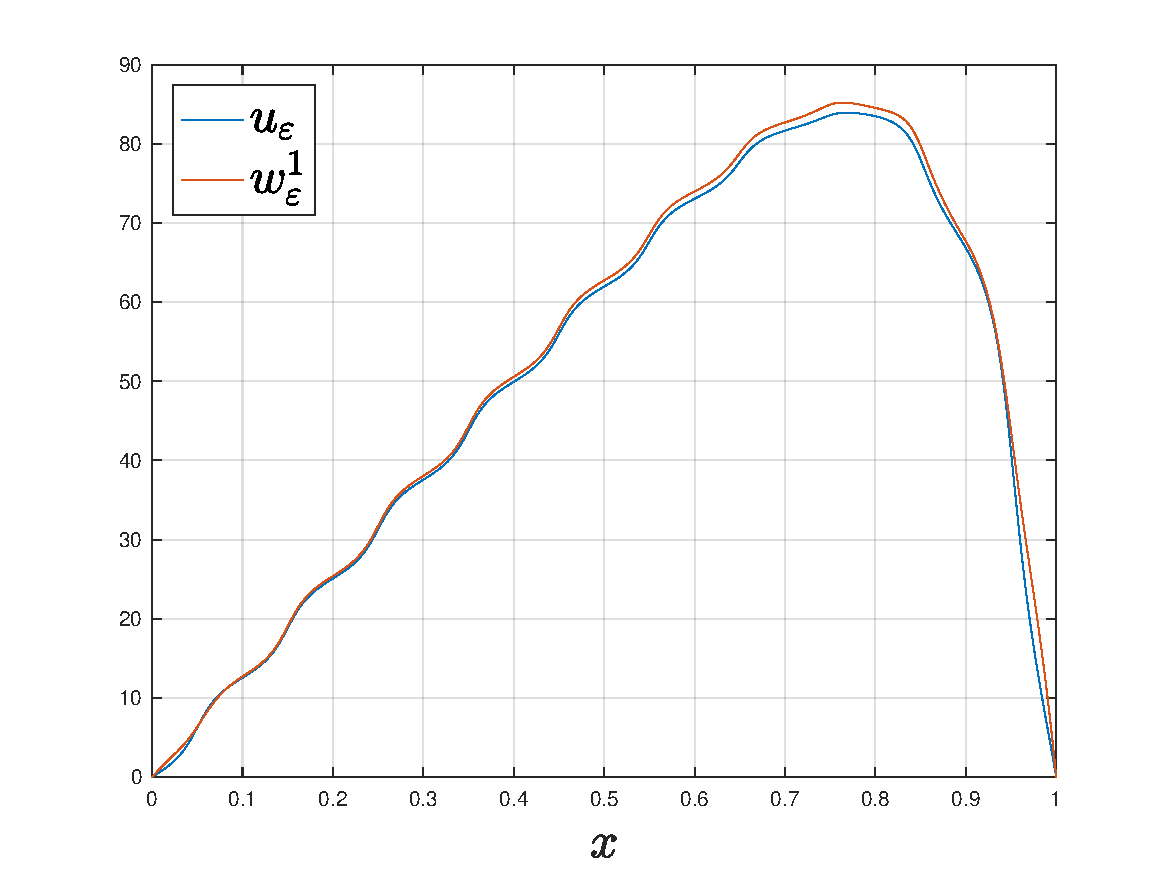
\includegraphics[width=\textwidth]{src/img/u_eps_w_1_eps_2.pdf}
        \caption{$\varepsilon = 0.1$}
    \end{subfigure}
    \begin{subfigure}[b]{0.5\textwidth}
        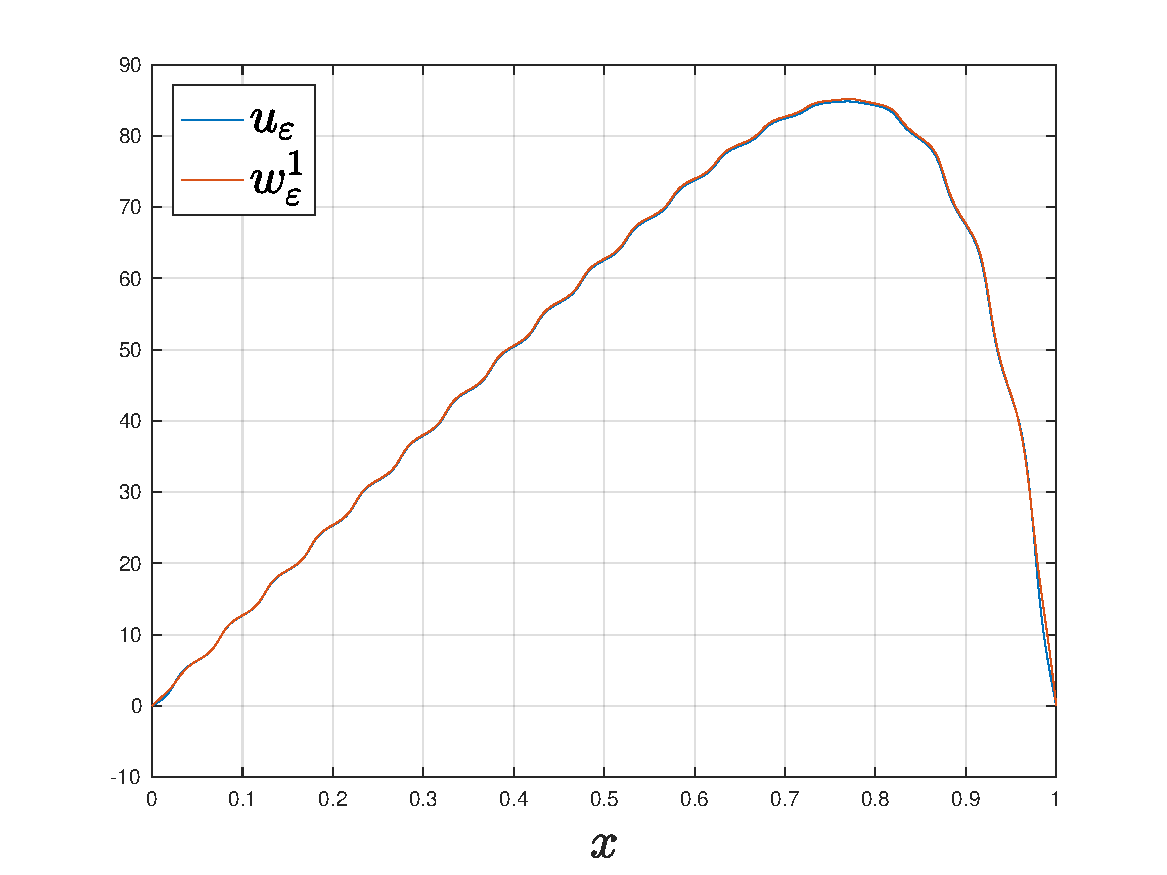
\includegraphics[width=\textwidth]{src/img/u_eps_w_1_eps_3.pdf}
        \caption{$\varepsilon = 0.05$}
    \end{subfigure}
    ~ %add desired spacing between images, e. g. ~, \quad, \qquad, \hfill etc. 
      %(or a blank line to force the subfigure onto a new line)
    \begin{subfigure}[b]{0.5\textwidth}
        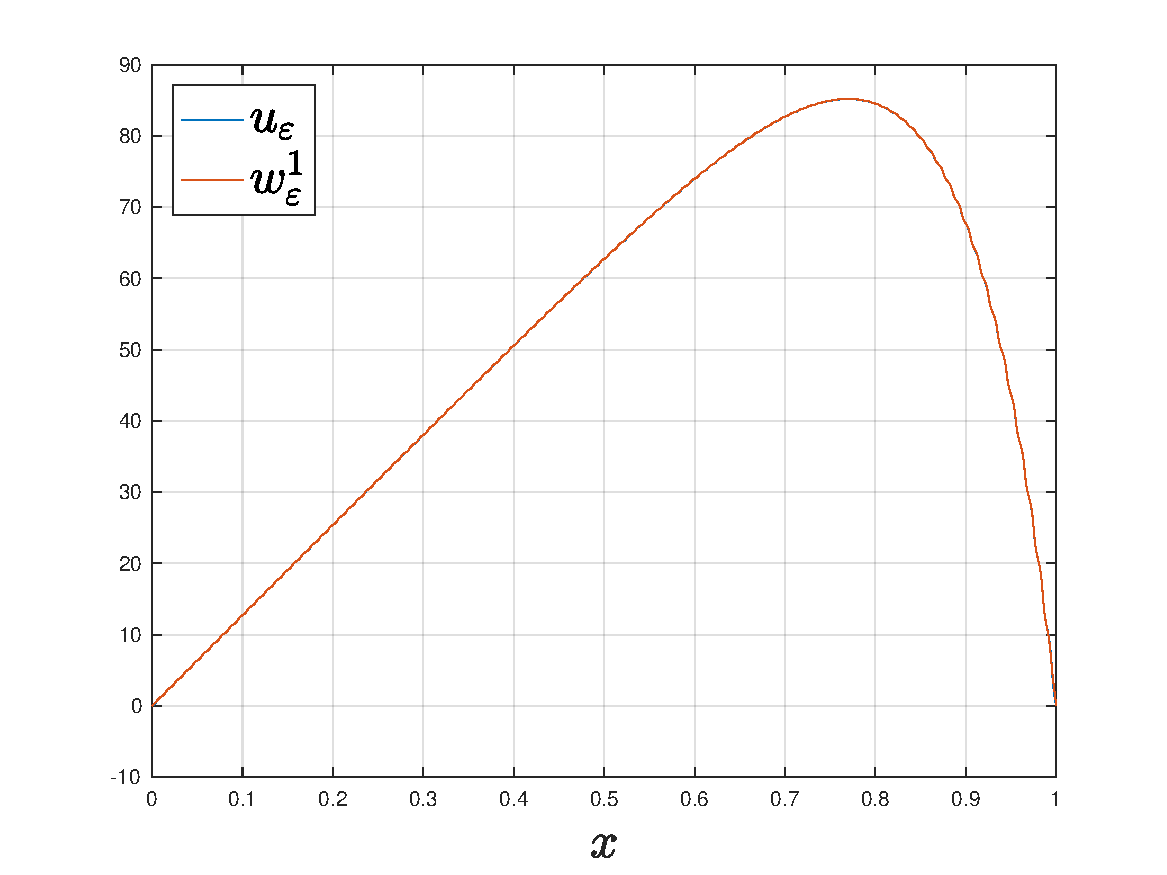
\includegraphics[width=\textwidth]{src/img/u_eps_w_1_eps_4.pdf}
        \caption{$\varepsilon = 0.01$}
    \end{subfigure}
    \caption{Plot of the approximations $w_\varepsilon^1$ of $u_\varepsilon$ for certain values of $\varepsilon$.}
    \label{fig:ex_2_plots}
	\end{figure}
	
	Now we want to numerically check the error estimate
	\begin{equation}
	\norm[0]{u_\varepsilon - w_\varepsilon^1}_{H^1(\Omega)} \leq c \sqrt{\varepsilon}.
	\end{equation}
	For that we have to calculate $(w_\varepsilon^1)'$ which involves $\psi_\varepsilon'$. This is the only difficult task. Using the notion of weak derivatives and $\min(f,g) = f + g - \abs[0]{f - g}$ we get that
	\begin{equation}
	\boxed{\psi_\varepsilon'(x) = -\frac{1}{2\varepsilon}\sgn(2x - 1)\del[2]{1 + \sgn\del[2]{1 - \frac{1}{2\varepsilon}(1 - \abs[0]{2x - 1})}}.}
	\end{equation}
	
	In figure \ref{fig:ex_2_plots_d} we see the approximation of $u_\varepsilon'$ by $(w_\varepsilon^1)'$ for certain values of $\varepsilon$. One observes that the approximations are not as quite as good as the one of $u_\varepsilon$ by $w_\varepsilon^1$.
	
	\begin{figure}[h!tb]
    \centering
    \begin{subfigure}[b]{0.5\textwidth}
        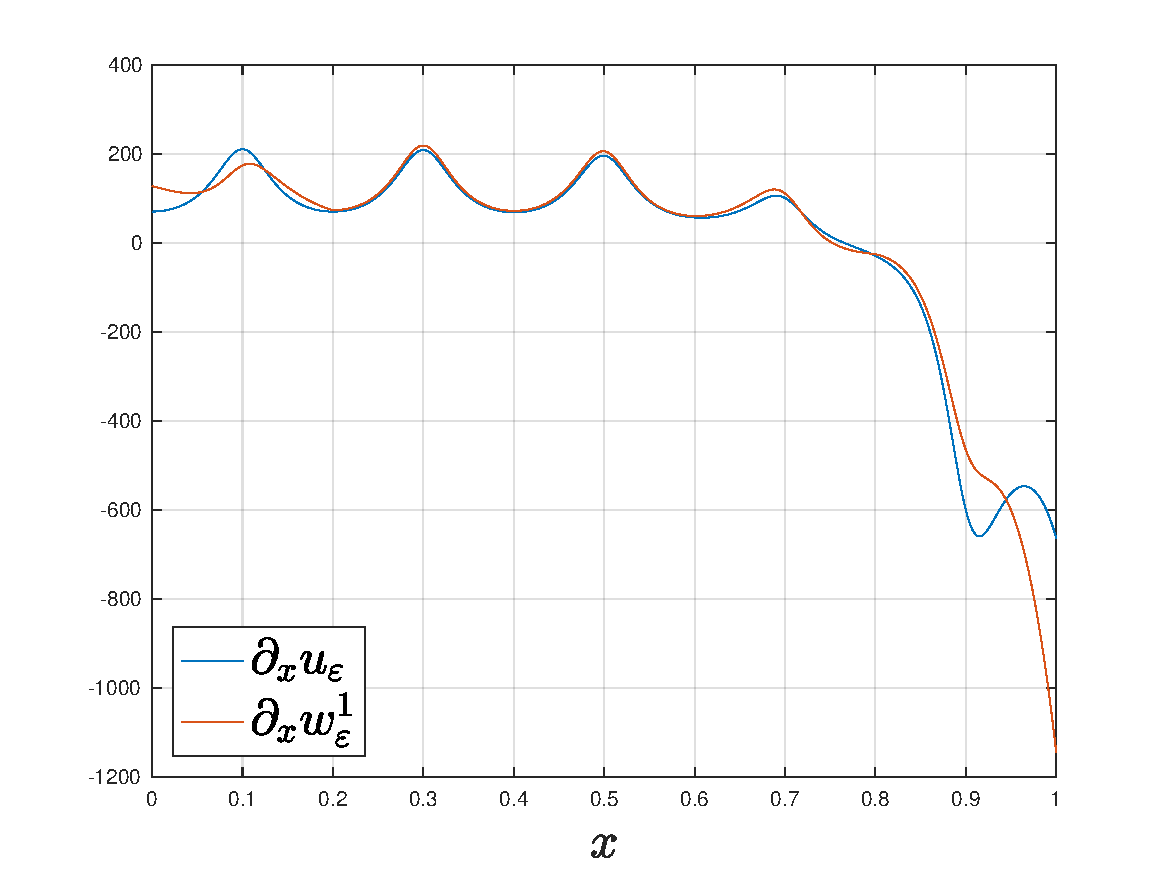
\includegraphics[width=\textwidth]{src/img/du_eps_dw_1_eps_1.pdf}
        \caption{$\varepsilon = 0.2$}
    \end{subfigure}
    ~ %add desired spacing between images, e. g. ~, \quad, \qquad, \hfill etc. 
      %(or a blank line to force the subfigure onto a new line)
    \begin{subfigure}[b]{0.5\textwidth}
        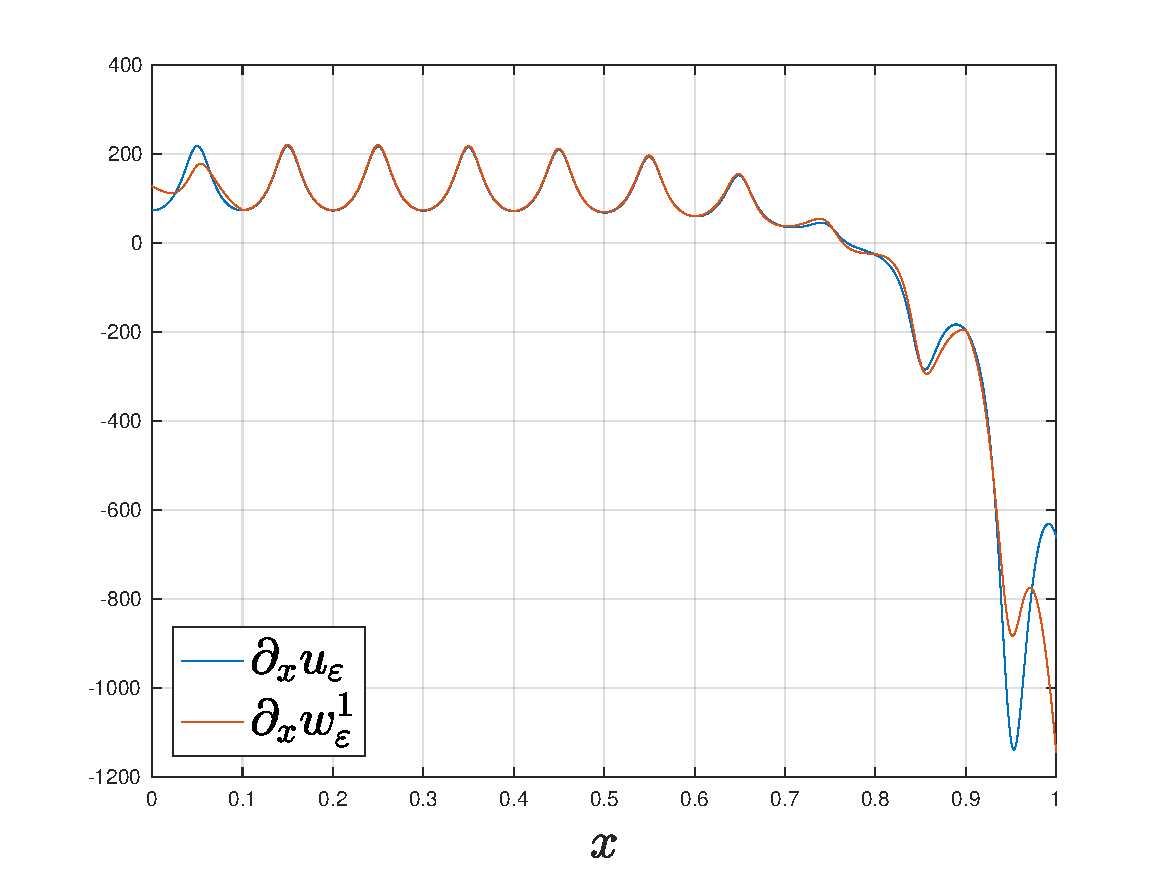
\includegraphics[width=\textwidth]{src/img/du_eps_dw_1_eps_2.pdf}
        \caption{$\varepsilon = 0.1$}
    \end{subfigure}
    \begin{subfigure}[b]{0.5\textwidth}
        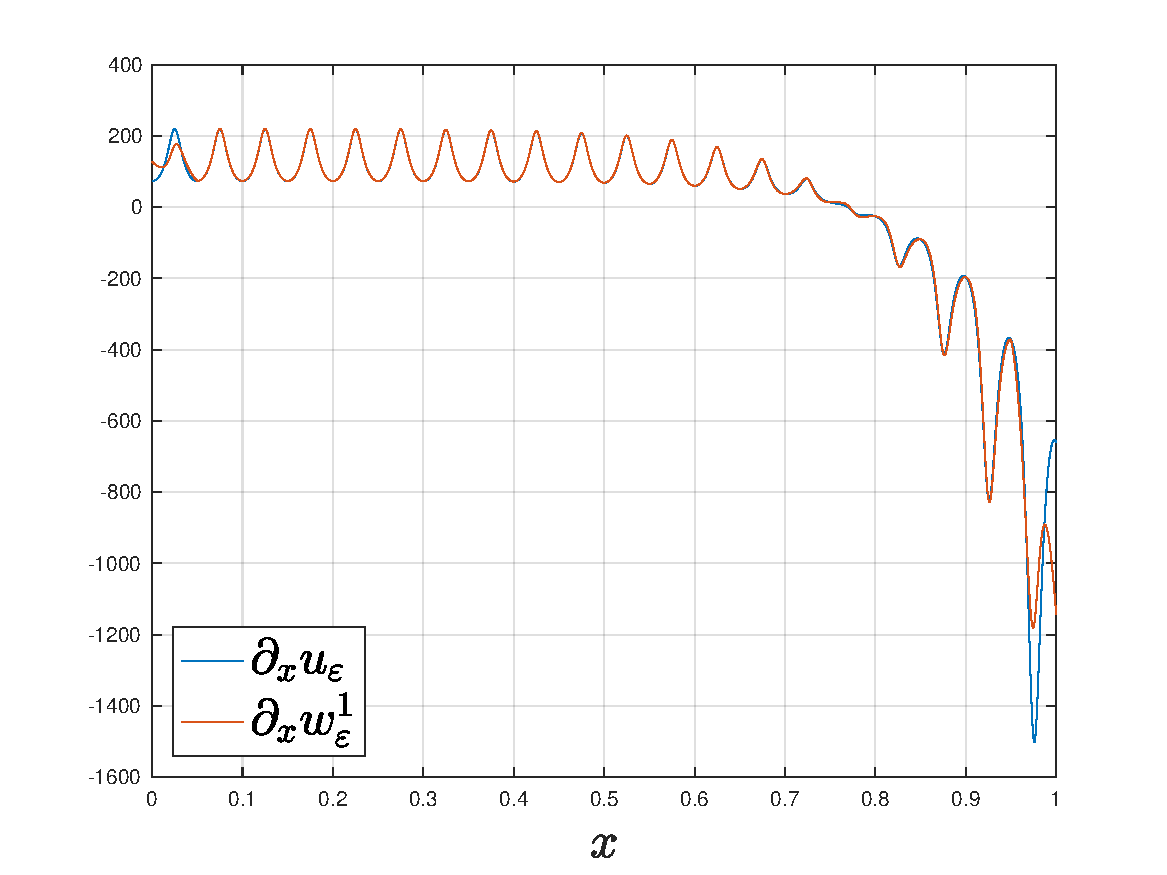
\includegraphics[width=\textwidth]{src/img/du_eps_dw_1_eps_3.pdf}
        \caption{$\varepsilon = 0.05$}
    \end{subfigure}
    ~ %add desired spacing between images, e. g. ~, \quad, \qquad, \hfill etc. 
      %(or a blank line to force the subfigure onto a new line)
    \begin{subfigure}[b]{0.5\textwidth}
        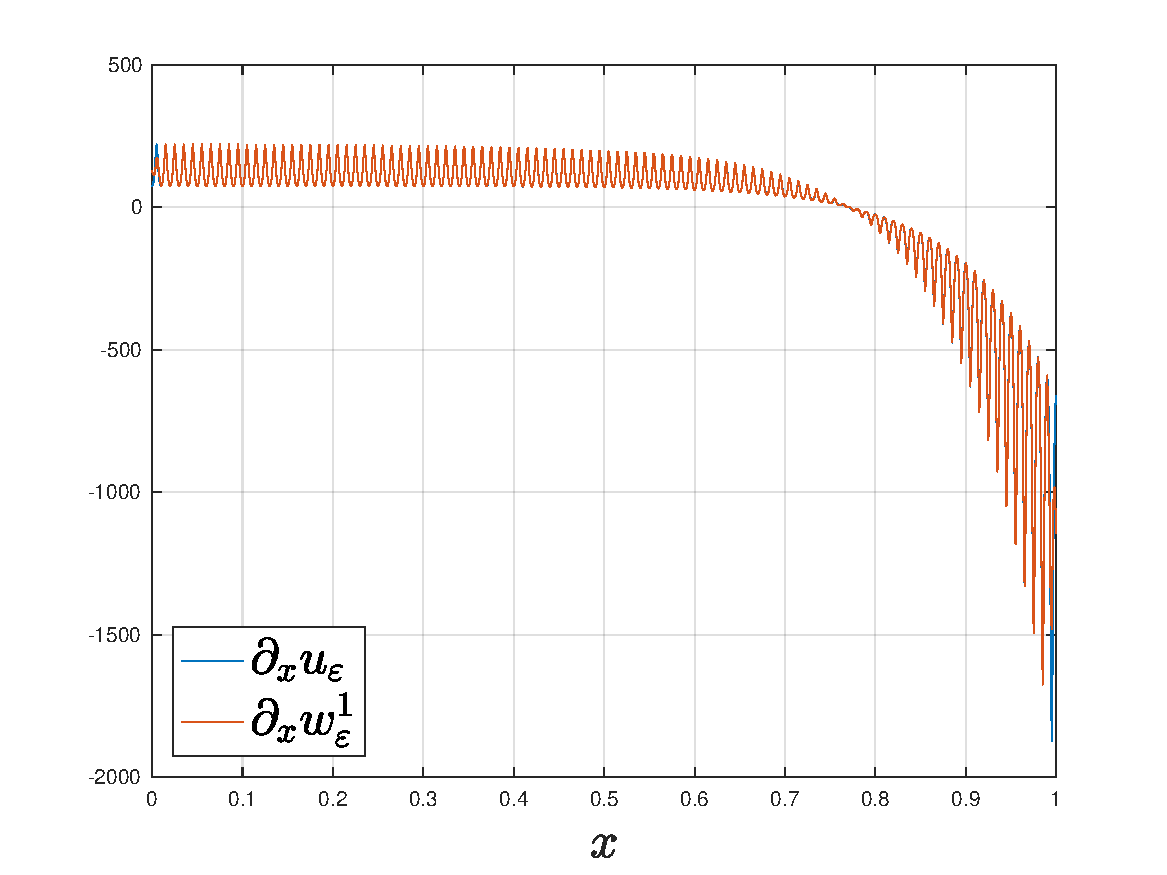
\includegraphics[width=\textwidth]{src/img/du_eps_dw_1_eps_4.pdf}
        \caption{$\varepsilon = 0.01$}
    \end{subfigure}
    \caption{Plot of the approximations $(w_\varepsilon^1)'$ of $u_\varepsilon'$ for certain values of $\varepsilon$.}
    \label{fig:ex_2_plots_d}
	\end{figure}
	
	\begin{figure}[h!tb]
	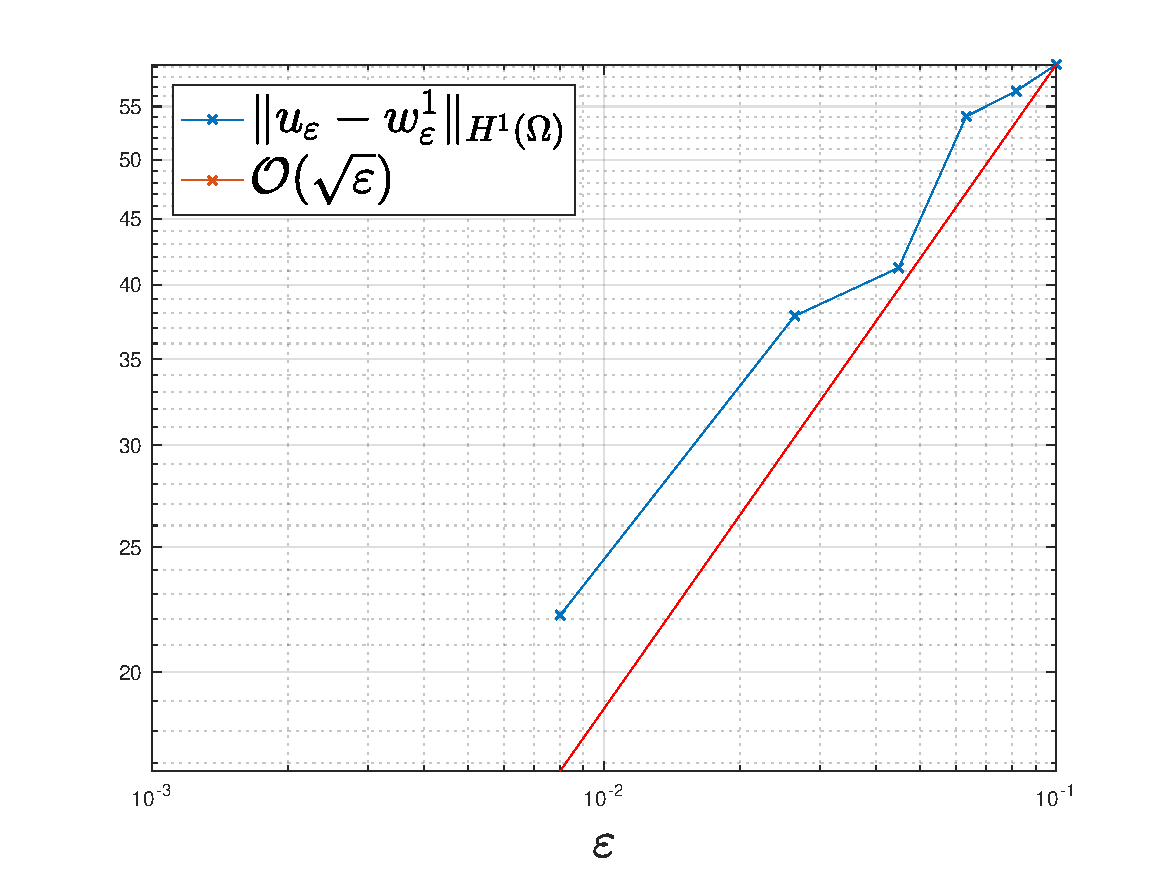
\includegraphics[width=\textwidth]{src/img/error.pdf}
	\caption{Plot of the error $\norm[0]{u_\varepsilon - w_\varepsilon^1}_{H^1(\Omega)}$.}
	\label{fig:error}
	\end{figure}
\end{example}
%Appendix
\appendix

\section{Listings}
\lstinputlisting{src/example.m}

\printbibliography
\end{document}
